\documentclass{article}
\usepackage[utf8]{inputenc}
\usepackage{multirow}
\usepackage{graphicx}
\usepackage[spanish]{babel}
\usepackage{amsmath}
\usepackage{xcolor}
\usepackage{mathrsfs}
\usepackage{fancyhdr}
\usepackage{multirow}
\usepackage{amssymb}
\usepackage[table,xcdraw]{xcolor}

\title{Reporte de Investigación}
\author{Facultad de Ciencias, Universidad Nacional Autonoma de México\\
Nadia Estefania Rosales Orozco, Almazan Borjas Jorge Iv\'an,\\ Osvaldo Mej\'ia Ochoa, Emiliano Guti\'errez Luengas}
\date{\today}

\begin{document}

\maketitle

\begin{abstract}
  En este estudio se buscó explorar los cambios en el desplazamiento de un projectil, con base en el cambio en la aceleración debido a un cambio en la fuerza gravitatoria. Se buscó ejemplificar, en pocas palabras, el desplazamiento del antedicho en diferentes planetas.
\end{abstract}


\section{Introducci\'on}
La mec\'anica cl\'asica fue, durante mucho tiempo, la rama de la f\'isica principal enfocada en estudiar los fen\'omenos naturales. Con el paso del tiempo y la llegada de personas que revolucionar\'ian el panorama cient\'ifico, se empezaron a crear nuevos campos de esta ciencia, que permit\'ian un an\'alisis m\'as complejo de los fen\'omenos antes citados. Sin embargo, algunas f\'ormulas de la mec\'anica cl\'asica siguen siendo usadas por su practicidad y la precisi\'on de los valores obtenidos que, aunque no sea tan exacta como la de un valor obtenido por otros m\'etodos, su diferencia es dificlmente considerable (i.e. la diferencia entre valores obtenidos es insignificante).
Retomando lo dicho con anterioridad, valores como el desplazamiento de un objeto, su velocidad, el tiempo tomado en recorrer una distancia, o la acelerac\'on de este pueden ser obtenidos con formulas relativamente simples. Con base en esto, este proyecto busca obtener los valores para el desplazamiento final y el tiempo de un proyectil disparado a una velocidad a criterio de los investigadores. Se evaluará el cambio que esas dos variables presenten con aceleraciones diferentes y, con el fin de simular este escenario, se buscar\'a representar el lanzamiento en diferentes planetas, siendo estos los escenarios.
Por facilitar los c\'alculos, se va a asumir que no hay corrientes de viento o fuerzas externas, m\'as all\'a de la gravedad.


\section{Objetivos}
\textbf{Objetivo general.} Evaluar los efectos de la gravedad de un planeta sobre el lanzamiento de un proyectil, con el fin de ajustar los parámetros necesarios para lograr un alcance en distancia esperado.\\ \\
\textbf{Objetivos específicos:} 
\begin{enumerate}
    \item Crear un código en python que de los valores de la variables alcance máximo en x,y, según los valores de gravedad para cada uno de los planetas del sistema solar.
    \item Comparar los valores de alcance y la relación con las masas de cada planeta
\end{enumerate}

\section{Hip\'otesis }
Se espera que los lanzamientos en los planetas con mayor masa tengan un alcance menor en comparacion con los de menor masa que se espera que tengan un alcance mayor.
 
\section{Desarrollo Experimental}
Primeramente, debido a la inaccesibilidad a equipo de laboratorio y nuestra incapacidad de manejarlo correctamente, se desarroll\'o el experimento con base en un código de Python.


Se dise\~no un entorno def que, al insertar los valores de la velocidad incial y la aceleraci\'on para cada escenario, regresa los valores en los que la altura es cero. Igualmente, el c\'odigo permite obtener la altura del proyectil para cualquier punto. Dicho de otra forma, permite encontrar la imagen de la funci\'on para cualquier valor de x.

\begin{figure}[h!]
    \centering
    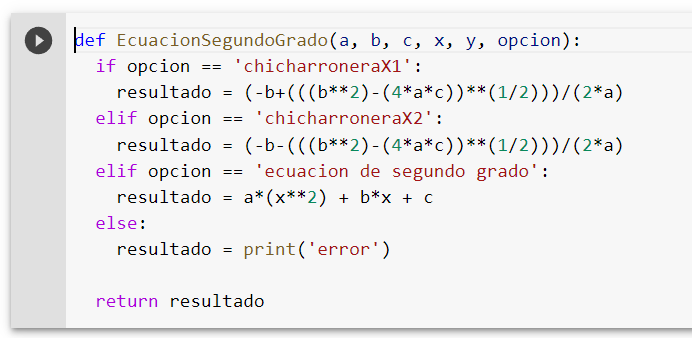
\includegraphics[scale=0.45]{Entorno_def.png}
    \caption{Entorno def}
    \label{fig:Entorno_def.}
\end{figure}

Para el experimento, se consideró a la velocidad inicial como 140, elevado a un \'angulo de 30 grados con respecto  a la horizontal. De forma que:

\begin{align*}
    Vt &= 140 m/s\\
    Vy &= 70 m/s\\
    Vx &= 121.24 m/s
\end{align*}

De manera que el tiempo tomado para que el proyectil cayera de nuevo al suelo queda de la siguiente forma:

\begin{table}[h]
\centering
\begin{tabular}{|c|c|c|c|}
\hline
Planeta   & \begin{tabular}[c]{@{}c@{}}Vx\\ m/s\end{tabular} & \begin{tabular}[c]{@{}c@{}}Vy\\ m/s\end{tabular} & \begin{tabular}[c]{@{}c@{}}t\\ s\end{tabular} \\ \hline
Mercurio  & \multirow{8}{*}{121.24}                          & \multirow{8}{*}{70}                              & 37.83783783783784                             \\ \cline{1-1} \cline{4-4} 
Venus     &                                                  &                                                  & 15.783540022547916                            \\ \cline{1-1} \cline{4-4} 
Tierra    &                                                  &                                                  & 14.271151885830784                            \\ \cline{1-1} \cline{4-4} 
Marte     &                                                  &                                                  & 37.735849056603776                            \\ \cline{1-1} \cline{4-4} 
J\'upiter &                                                  &                                                  & 5.647438483259379                             \\ \cline{1-1} \cline{4-4} 
Saturno   &                                                  &                                                  & 13.409961685823756                            \\ \cline{1-1} \cline{4-4} 
Urano     &                                                  &                                                  & 15.783540022547916                            \\ \cline{1-1} \cline{4-4} 
Neptuno   &                                                  &                                                  & 12.556053811659192                            \\ \hline
\end{tabular}
\caption{Velocidad del componente en x, del componente en f(x), y tiempo tomado}
\label{tab:my-table}
\end{table}

Igualmente, los valores para aceleraci\'on seleccionados fueron los de los planetas del sistema solar. Estos fueron anotados en una tabla para uso posterior, como se puede observar en la imagen siguiente.\newpage

%El código de una tabla. Esta muestra los valores para la aceleración por gravedad para cada planeta.
\begin{table}[h]
\centering
\begin{tabular}{|c|c|}
\hline
\textbf{Planeta} & \textbf{\begin{tabular}[c]{@{}c@{}}Aceleraci\'on de Gravedad\\ $[m/s^2]$\end{tabular}} \\ \hline
Mercurio         & 3.7                                                                                              \\ \hline
Venus            & 8.87                                                                                             \\ \hline
Tierra           & 9.81                                                                                             \\ \hline
Marte            & 3.71                                                                                             \\ \hline
J\'upiter        & 24.79                                                                                            \\ \hline
Saturno          & 10.44                                                                                            \\ \hline
Urano            & 8.87                                                                                             \\ \hline
Neptuno          & 11.15                                                                                            \\ \hline
\end{tabular}
\caption{Valores para la aceleraci\'on por gravedad}
\label{tab:valores_aceleracion}
\end{table}

Una vez con el entorno def y los valores a usar establecidos, se crearon 8 celdas. En cada una se aplic\'o el entorno, mas con los valores respectivos para cada simulaci\'on. Su finalidad fue la de encontrar las raices de la par\'abola que traza el proyectil en cada escenario. La aceleraci\'on fue considerada negativa en cada caso, con el fin de simular la reducci\'on de la velocidad en la subida y el consecuente incremento de esta en la bajada.

Cabe notar que la par\'abola formada es simétrica, ya que el proyectil se dispara del suelo y se estrella con el antedicho. Por lo tanto, para encontrar la altura m\'axima, solamente cabe obtener el tiempo entre las ra\'ices, dividirlo entre dos, y reemplazar en la ecuaci\'on de desplazamiento original (la ecuaci\'on de la par\'abola).\\

\begin{figure}[h!]
    \centering
    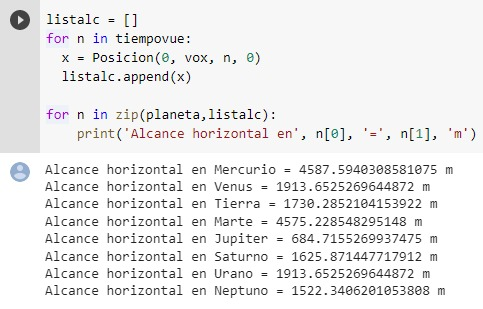
\includegraphics[scale=0.5]{alcance en x.jpeg}
    \caption{C\'odigo Utilizado para encontrar la distancia maxima}
    \label{fig:Codigo_Utilizado}
\end{figure}

\begin{figure}[h!]
    \centering
    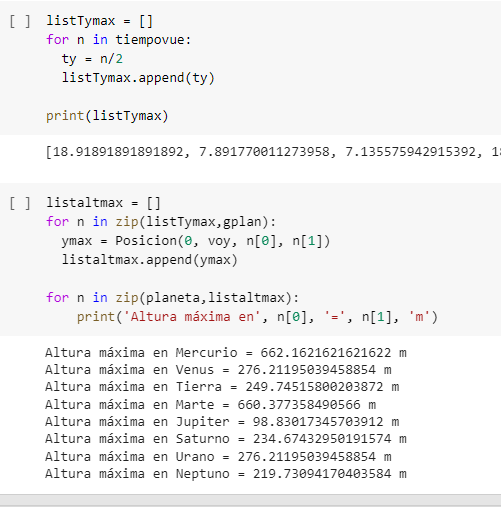
\includegraphics[scale=0.5]{listTymax.png}
    \caption{C\'odigo Utilizado para encontrar la altura maxima}
    \label{fig:Codigo_Utilizado}
\end{figure}



\newpage




\section{Resultados y An\'alisis de resultados}
%El código de una tabla. Muestra el desplazamiento máximo en "x" y en "y" para el proyectil.
\begin{table}[h!]
\centering
\begin{tabular}{|c|c|c|}
\hline
\textbf{Planeta} & \textbf{\begin{tabular}[c]{@{}c@{}}Desplazamiento M\'aximo en x\\ $[m]$\end{tabular}} & \textbf{\begin{tabular}[c]{@{}c@{}}Desplazamiento M\'aximo en f(x)\\ $[m]$\end{tabular}} \\ \hline
Mercurio         & 4587.459459459459                                                                     & 662.1621621621621                                                                        \\ \hline
Venus            & 1913.5963923337092                                                                    & 276.21195039458854                                                                       \\ \hline
Tierra           & 1730.2344546381241                                                                    & 249.7451580020387                                                                        \\ \hline
Marte            & 4575.094339622641                                                                     & 660.3756890271059                                                                        \\ \hline
J\'upiter        & 684.6954417103672                                                                     & 98.83017345703911                                                                        \\ \hline
Saturno          & 1625.823754789272                                                                     & 234.6743295019157                                                                        \\ \hline
Urano            & 1913.5963923337092                                                                    & 276.21195039458854                                                                       \\ \hline
Neptuno          & 1522.2959641255604                                                                    & 219.7309417040359                                                                        \\ \hline
\end{tabular}
\caption{Valores para el m\'aximo desplazamiento dado en x y en f(x)}
\label{tab:Desplazamiento_maximo}
\end{table}


Se puede observar, de manera esperada, una diferencia considerable entre el desplazamiento entre los planetas con menor fuerza gravitatoria y el desplazamiento dado en J\'upiter, el planeta con la mayor de estas. Igualmente, cabe recalcar que los tiempos tomados para la ca\'ida son mayores cuando la gravedad es m\'as d\'ebil.
\\
En orden descendente, el mayor alcance en ambos ejes se dio en Mercurio y Marte, seguido por Venus y Urano (coincidieron exactamente, a pesar de que su tamaño es diferente, el radio influye también, siendo más denso Venus por ser rocoso). Luego siguieron la Tierra, Neptuno, Saturno, y por último Júpiter. Es decir, si es lanzado un proyectil con la misma velocidad y ángulo, alcanzará más distancia en Mercurio, mientras que en Júpiter se requeriría una velocidad inicial mucho mayor para igualar la distancia alcanzada en Mercurio.

\section{Conclusiones}
Como se esperaba la hip\'otesis es acertada. Mientras más masa tenga un planeta afectara el desplazamiento de los proyectiles causando que su alcance sea menor en comparacion con un planeta de menor masa, pero no solo el tiempo que tarda en caer el proyectil es mayor cuando la gravedad es menor, y menor cuando la gravedad es mayor, esto claramente sucede por la aceleración de gravedad.\\
Notemos que el menor alcance se obtuvo en J\'upiter y el mayor en Mercurio, con 685 m en desplazamiento horizontal y 99 m de altura máxima, y 4587 m en desplazamiento horizontal y 662 m en altura m\'axima, respectivamente. Además, cabe mencionar que la gravedad de J\'upiter es 6.7 veces mayor a la de Mercurio, relacionadas con sus valores de masa y radio.

\begin{thebibliography}{X}
  \bibitem{Deplanetas} \textsc{Deplanetas}. (2020, 22 junio).
\textit{¿Cuál es la gravedad de los planetas del Sistema Solar?} (TELESCOPIOS DEPLANETAS.COM). https://deplanetas.com/cual-es-la-gravedad-de-los-planetas-del-sistema-solar/
\end{thebibliography}


\end{document}
